\documentclass[11pt]{article}
\usepackage{amsfonts,amsthm,amsmath,amssymb, hyperref, dsfont, enumitem, bbm}
\usepackage{array}
\usepackage{epsfig}
\usepackage{fullpage}
\usepackage{color}
\usepackage{epigraph}
\renewcommand{\epigraphflush}{center}
\usepackage[framemethod=tikz]{mdframed}
\usepackage{titlesec}
\usepackage{ellipsis}
\usepackage{subcaption}
\usepackage[normalem]{ulem}
\usepackage{todonotes}


\titleformat{\chapter}[display]
  {\normalfont\bfseries}{}{0pt}{\Huge}

\newif\ifdetails % fill in details that are omitted in lecture handout version


\newcommand{\qn}[1]{\todo[inline, color=brown!30]{Quynh: #1}}
\newcommand{\duc}[1]{\todo[inline, color=red!30]{Duc: #1}}

\detailstrue %Change to detailsfalse when removing text

\begin{document}

%% Courtesy: Daniel Spielman, via Madhu Sudan --> Chi-Ning Chou --> Anurag Anshu

\theoremstyle{plain}
\newtheorem{theorem}{Theorem}[section]
\newtheorem{lemma}[theorem]{Lemma}
\newtheorem{example}[theorem]{Example}
\newtheorem{corollary}[theorem]{Corollary}
\theoremstyle{definition}
\newtheorem{definition}[theorem]{Definition}
\newtheorem*{mydefinition}{Definition}
\newtheorem{claim}[theorem]{Claim}
\newtheorem{fact}[theorem]{Fact}
\newtheorem{remark}[theorem]{Remark}
\newtheorem{exercise}[theorem]{Exercise}

%Left and right brackets
\newcommand {\br} [1] {\ensuremath{ \left( #1 \right) }}
\newcommand {\Br} [1] {\ensuremath{ \left[ #1 \right] }}


%Quantum notations
\newcommand {\norm}[1]{{\| #1 \|}}  
\newcommand {\bra} [1] {\ensuremath{ \left\langle #1 \right| }}
\newcommand {\ket} [1] {\ensuremath{ \left| #1 \right\rangle }}
\newcommand {\ketbratwo} [2] {\ensuremath{ \left| #1 \middle\rangle \middle\langle #2 \right| }}
\newcommand {\ketbra} [1] {\ketbratwo{#1}{#1}}
\newcommand{\braket}[2]{\langle#1|#2\rangle}
\newcommand{\Tr}[1]{\mathrm{Tr}\left(#1\right)}
\newcommand{\tr}[2]{\mathrm{Tr}_{#1}\left(#2\right)}
\newcommand{\PE}{\mathrm{PE}}
\newcommand{\EPR}{\mathrm{EPR}}
\newcommand{\CNOT}{\mathrm{CNOT}}
\newcommand{\CZ}{\mathrm{CZ}}

%Generic math symbols
\newcommand {\eps} {\varepsilon}
\newcommand{\tO}{\tilde{O}}
\newcommand{\ind}[1]{\mathrm{Ind}\left(#1\right)}
\newcommand {\id}{\mathds{1}}
\newcommand{\bitn}[1]{\ensuremath{\{0,1\}^{#1}}}
\newcommand{\bitone}{\ensuremath{\{0,1\}}}
\newcommand{\swp}{\mathrm{\textbf{Swap}}}

% Information theory and CS symbols
\newcommand {\prob} {\ensuremath{\mathrm{Prob}}}
\newcommand{\bigo}[1]{\mathcal{O}\left(#1\right)}
\newcommand{\omeg}[1]{\Omega\left(#1\right)}
\newcommand{\expec}{\mathbb{E}}
\newcommand{\relent}[2]{\mathrm{D}\left(#1\|#2\right)}
\newcommand{\KL}[2]{\mathrm{D}_{KL}\left(#1\|#2\right)}
\newcommand{\mutinf}[2]{\mathrm{I}\left(#1:#2\right)}
\newcommand{\condmutinf}[3]{\mathrm{I}\left(#1:#2|#3\right)}
\newcommand{\condent}[2]{\mathrm{S}\left(#1|#2\right)}
\newcommand{\ent}[1]{\mathrm{S}\left(#1\right)}
\newcommand{\cla}{\text{classical}}
\newcommand{\qua}{\text{quantum}}
\newcommand{\sym}{\textsf{sym}}

%Statistical measures
\newcommand{\F}{\mathrm{F}}
\newcommand{\tv}{\mathrm{TV}}
\newcommand{\Hol}{\mathrm{Hol}}
\newcommand{\hel}{\mathrm{Hd}}
\newcommand{\pur}{\mathrm{Pur}}
\newcommand{\scs}{\mathrm{succ}}
\newcommand{\err}{\mathrm{err}}
\newcommand{\can}{\mathrm{can}}
\newcommand{\Var}{\mathrm{Var}}

%Fancy alphabets
\def\cA{\mathcal{A}}
\def\cB{\mathcal{B}}
\def\cC{\mathcal{C}}
\def\cD{\mathcal{D}}
\def\cE{\mathcal{E}}
\def\cF{\mathcal{F}}
\def\cG{\mathcal{G}}
\def\cH{\mathcal{H}}
\def\cL{\mathcal{L}}
\def\cM{\mathcal{M}}
\def\cO{\mathcal{O}}
\def\cP{\mathcal{P}}
\def\cR{\mathcal{R}}
\def\cS{\mathcal{S}}
\def\cT{\mathcal{T}}
\def\cX{\mathcal{X}}
\def\N{\mathbb{N}}
\def\Z{\mathbb{Z}}



%%%%%%%%%%%%%%%%%%%%%%%%%%%%%%%%%%%%%%%%%%%%% 
%Commands below can be ignored by the students  
%%%%%%%%%%%%%%%%%%%%%%%%%%%%%%%%%%%%%%%%%%%%%
% Header
\newcommand{\handout}[5]{
   \renewcommand{\thepage}{#1-\arabic{page}}
   \noindent
   \begin{center}
   \framebox{
      \vbox{
    \hbox to 6.3in { {\bf #1}
     	 \hfill {\it #3} }
       \vspace{4mm}
       \hbox to 6.3in { {\Large \hfill #5  \hfill} }
       \vspace{2mm}
       \hbox to 6.3in { {\it #2 \hfill #4} }
      }
   }
   \end{center}
   \vspace*{4mm}
}

\newcommand{\lecture}[4]{\handout{#1}{#2}{Lecturer:
#3}{Scribe: #4}{Lecture #1}}



%Editing commands
\newcommand{\edit}[2]{\st{#1}\hspace{0.05in}\textcolor{blue}{#2}}
\newcommand{\suppress}[1]{}

\newcommand{\anote}[1]{{\color{red} \textbf{Anurag's note:} #1}}
\newcommand{\qnote}[1]{{\color{red} \textbf{Quynh's note:} #1}}
\newcommand{\hkn}[1]{{\color{orange} \textbf{Nguyen nu:} #1}}


%Itemizing and Equation shorthands
\newcommand{\beit}{\begin{itemize}}
\newcommand{\enit}{\end{itemize}}
\newcommand{\been}{\begin{enumerate}}
\newcommand{\enen}{\end{enumerate}}
\newcommand{\beq}{\begin{equation}}
\newcommand{\enq}{\end{equation}}
\newcommand{\beqst}{\begin{equation*}}
\newcommand{\enqst}{\end{equation*}}
\newcommand{\beqar}{\begin{eqnarray}}
\newcommand{\enqar}{\end{eqnarray}}
\newcommand{\beqarst}{\begin{eqnarray*}}
\newcommand{\enqarst}{\end{eqnarray*}}




\handout{SEAS 2025 - Adapted from MIT 18.650 }{{\bf July ..., 2025}}{Instructor: Duc Hoang }{TA: }{Statistics 3: Linear Regression}

\section{Introduction to Linear Models}

When we talk about a \textbf{linear model} in statistics, we’re referring to any model that assumes a straight-line relationship somewhere in the system. The most common example is what you probably already know—\text{linear regression}—where we fit a straight line to data to understand how variables are related.


So why do we care about models being ``linear''? Because linear models are mathematically elegant—they’re easier to work with, easier to interpret, and they often let us simplify very complex problems without losing too much accuracy. In other words, they give us powerful tools to model the real world without getting lost in mathematical chaos.

\vspace{1em}

In this lecture, we will introduce the concept of linear models, with a special focus on one of the most important and widely used cases: \textbf{linear regression}.

\section{Definitions and main concepts}
In regression, we predict the value of a \emph{response variable} $Y\in\R$ based on a \emph{feature vector} or \emph{predictor} $X\in\R^k$.
\begin{example}
The feature vector $X$ and response $Y$ could be e.g.
$$X=
\begin{pmatrix}\text{weight}\\\text{age}\\ \text{salary}\\\text{GPA}\end{pmatrix},\quad Y=\text{IQ}.
$$
Another example of a $Y$ is whether or not the person will default on a credit. In this case $Y$ only takes the value 0 or 1.
\end{example}


\noindent \textbf{Goal:} predict $Y$ given $X$, or understand how $Y$ changes with $X$. (In particular, understand which of the features in $X$ are particularly relevant for predicting $Y$.)\\

\noindent\textbf{Difficulty}: For each fixed $X=x$, there is a whole probability distribution $Y|X=x$. For example, we could have $Y|X=x\sim\mathcal N(f(x),\sigma^2)$. It is not realistic to assume that there is a function $f(x)$ such that knowing $X=x$ implies $Y=f(x)$ exactly. \\

\noindent\textbf{Best prediction property:} Although we cannot hope to find a function $f$ such that $Y=f(X)$ exactly, we can look for $f$ which minimizes the expected error $\E[(Y-f(X))^2]$. To minimize this expectation, first note that
$$\E[(Y-f(X))^2] = \E[\E[(Y-f(X))^2\mid X]]$$ by the tower property of conditional expectation. We can now minimize the inner expectation for each possible $X=x$: %Now we'll just minimize
$$\min_{f(x)}\E[(Y-f(x))^2\mid X=x] = \min_{a}\E[(Y-a)^2\mid X=x].$$ In other words, $f(x)$ is just the value $a$ that minimizes $h(a)=\E[(Y-a)^2\mid X=x]$. We minimize $h$ by setting the derivative to zero:
\beqsn
0=h'(a) = &2\E[Y-a\mid X=x] = 2(\E[Y\mid X=x] - a)\\
&\Rightarrow a=\E[Y\mid X=x].
\eeqsn

The minimizing function is $f(x)=\E[Y\mid X=x]$.
\begin{defn}{Regression function}{}
Given a random vector $X\in\R^k$ and a random variable $Y\in\R$, the function $f:\R^k\to\R$ given by
$$f(x)=\E[Y\mid X=x]$$ is called the regression function of $Y$ onto $X$.
\end{defn}
\begin{remark}
The definition extends to multivariate $Y$. %(You might want to simultaneously predict, say, two quantities from the features)
\end{remark}

In practice, we only get to observe pairs $(X_i, Y_i)$, as in Figure~\ref{fig:scatterreg}. So of course, we cannot perfectly compute the regressor function $f(x)=\E[Y|X=x]$ --- there are lots of $x$'s for which we don't get to observe even a single $y$! 

It's also important to keep in mind that even if we \emph{could} perfectly compute $\E[Y|X=x]$, this expectation does not fully capture the distribution $Y\mid X=x$. An alternative to vanilla regression (finding the mean $f(x)$) is quantile regression, which gives a confidence band around the mean. 

%Assume we observe $(X_i, Y_i)$, $i=1,\dots, n$, where $(X_1, Y_1)$, $(X_2, Y_2)$. .... are i.i.d. (draw scatterplot with nonlinear relationship). E.g. GPA of typical MIT student with time. Remember the best function is $\E[Y\mid X=x]=f(x)$. It's the solid curve. 

%Note there's a whole distribution $Y\mid X=x$! The expectation only describes a single point of this distribution. 
%May also want to get quantiles! A whole confidence band. (Quantile regression).
 \begin{figure}[h]
%\vspace{-30pt}
\center
    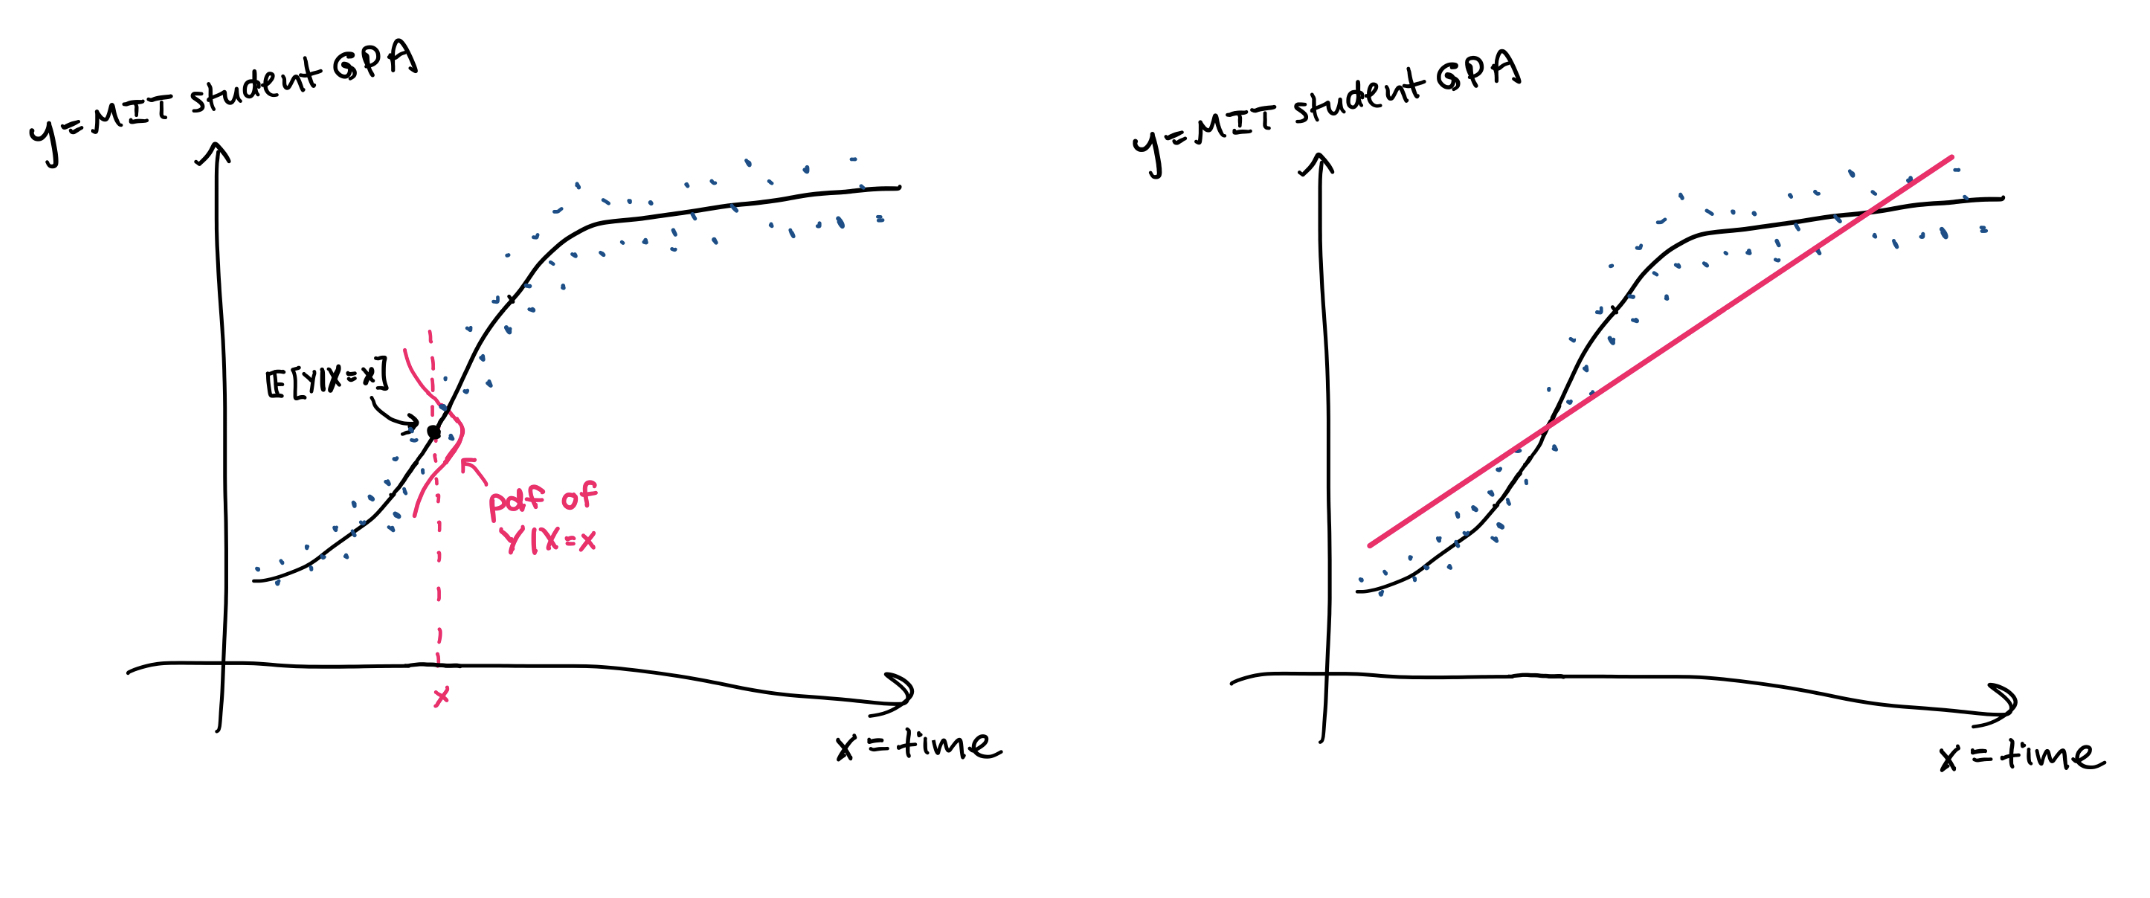
\includegraphics[scale=0.19]{figures/lec3_scatterreg.png}
    \caption{A scatterplot of observations $(X_i,Y_i)$ (blue points). In the lefthand plot, the solid black curve depicts the expectation $\E[Y|X=x]$. In the righthand plot, the pink line denotes a linear fit to the data.}
        \label{fig:scatterreg}
\end{figure}
\section{Linear regression.} In linear regression, we make the assumption that $f(x)=\E[Y|X=x]$ is \emph{linear in $x$}, i.e. of the form
$$f(x) =\E[Y|X=x]= x^\tr \beta$$ for some unknown ground truth $\beta=\beta^*\in\R^k$. To find an estimator of $\beta^*$ we'll use the MLE. To compute the MLE, we first need to assume a parametric form for the distribution of $Y|X=x$. We'll use our favorite distribution, the Gaussian.\\


\noindent\textbf{Assumption G:} For some unknown $\beta^*$ and (usually known) $\sigma^2$, it holds 
$$Y\mid X=x\sim\mathcal N(x^\tr \beta^*, \sigma^2).$$ Assumption G actually incorporates three separate assumptions:
\begin{enumerate}
\item $Y\mid X=x$ is $\mathcal N(f(x),\sigma^2(x))$, i.e. some generical Gaussian distribution.
\item The mean function is linear: $f(x)=x^\tr \beta^*$
\item The variance function is constant: $\sigma^2(x)=\sigma^2$ for all $x$.
\end{enumerate}
\begin{remark}
The last assumption, that $\sigma^2(x)$ is constant for all $x$, is know as homoskedastic regression, as opposed to heteroskedastic regression.
\end{remark}

Now that we have a statistical model, we can write down the log likelihood $\ell_n(\beta)$ and use it to compute the MLE $\hat\beta^\mle$.
$$\ell_n(\beta) = \sum_{i=1}^n\log\l(\frac{1}{\sigma\sqrt{2\pi}}\exp\l(-\frac{(Y_i-X_i^\tr \beta)^2}{2\sigma^2}\r)\r) = -\frac{1}{2\sigma^2}\sum_{i=1}^n(Y_i-X_i^\tr \beta)^2+\mathrm{const}.$$ Since maximizing $\ell_n$ is equivalent to minimizing $-\ell_n$, we see that the MLE is given by
\beq\label{MLEmin}\hat\beta^\mle = \argmin_{\beta\in\R^k}\sum_{i=1}^n(Y_i-X_i^\tr \beta)^2.\eeq
\begin{remark}
We could get to the same formula for the MLE by minimizing the expected error $\E[(Y-f(X))^2]$ over all linear $f$:
$$\min_{f\text{ linear}}\E[(Y-f(X))^2]=\min_\beta\E[(Y-X^\tr \beta)^2]\stackrel{\text{plug-in rule}}{\rightsquigarrow}\min_\beta\sum_{i=1}^n(Y_i-X_i^\tr \beta)^2.$$
This has.to do with the fact that minimizing a quadratic loss is equivalent to maximizing a Gaussian probability.
\end{remark}

\noindent\textbf{Exercise} Suppose that instead of having a constant $\sigma^2$, we assumed the variance was given by some known function $\sigma^2(x)$. In this case, what is the MLE $\hat\beta^\mle$? 

\subsection{Closed form solution for least squares}Let's find a closed form solution to $\hat\beta^\mle$, the minimizer in~\eqref{MLEmin}. To do this we'll need some matrix calculus. First, write all the $Y_i$'s into a vector:
$$Y=\begin{pmatrix}Y_1\\ Y_2\\\vdots\\Y_n
\end{pmatrix}\in\R^n.$$ Next, put the $X_i$'s as rows in the following matrix:
$$\XX=\begin{pmatrix} \text{---} & X_1^\tr &  \text{---}  \\  \text{---}  & X_2^\tr&  \text{---}  \\ & \vdots &\\  \text{---}  & X_n^\tr &  \text{---} 
\end{pmatrix}\in\R^{n\times k}.$$ We can now write the minimization problem~\eqref{MLEmin} as
$$\min_\beta\sum(Y_i-X_i^\tr \beta)^2 =\min_\beta\|Y-\XX\beta\|^2$$ We set the gradient with respect to $\beta$ to zero to get
$$2\XX^\tr (Y-\XX\beta)=0\implies \XX^\tr Y = \XX^\tr \XX\beta\implies\hat\beta^{\text{LS}} = (\XX^\tr \XX)^{-1}\XX^\tr Y,$$ where the LS stands for least squares (but it's also the MLE). \\

\noindent\textbf{Interpretation of the LS solution.} Note that if we multiply both sides of $\hat\beta^{\text{LS}}$ by $\XX$, we get
$$\XX\hat\beta = \XX(\XX^\tr \XX)^{-1}\XX^\tr Y=PY,\qquad P:=\XX(\XX^\tr \XX)^{-1}\XX^\tr .$$ The matrix $P$ is a \emph{projection matrix}: it satisfies $P^\tr =P$ and $P^2=P$. Therefore, the fact that $\XX\hat\beta=PY$ shows that $\XX\hat\beta$ is the projection of $Y$ onto span$(\XX)$, the linear space spanned by the columns of $\XX$. 

In other words, the formula for $\hat\beta^{\text{LS}}$ is implicitly encoding two steps: first, we find the closest point to $Y$ in the column span of $\XX$ (the projection of $Y$). This is the point $PY$. Since $PY$ lies in the column span, it is by definition given by some linear combination of the columns of $\XX$. Therefore, the second step is to identify the coefficients of this linear combination --- these are precisely the entries of $\hat\beta^{\text{LS}}$.

 \begin{figure}[h]
%\vspace{-30pt}
\center
    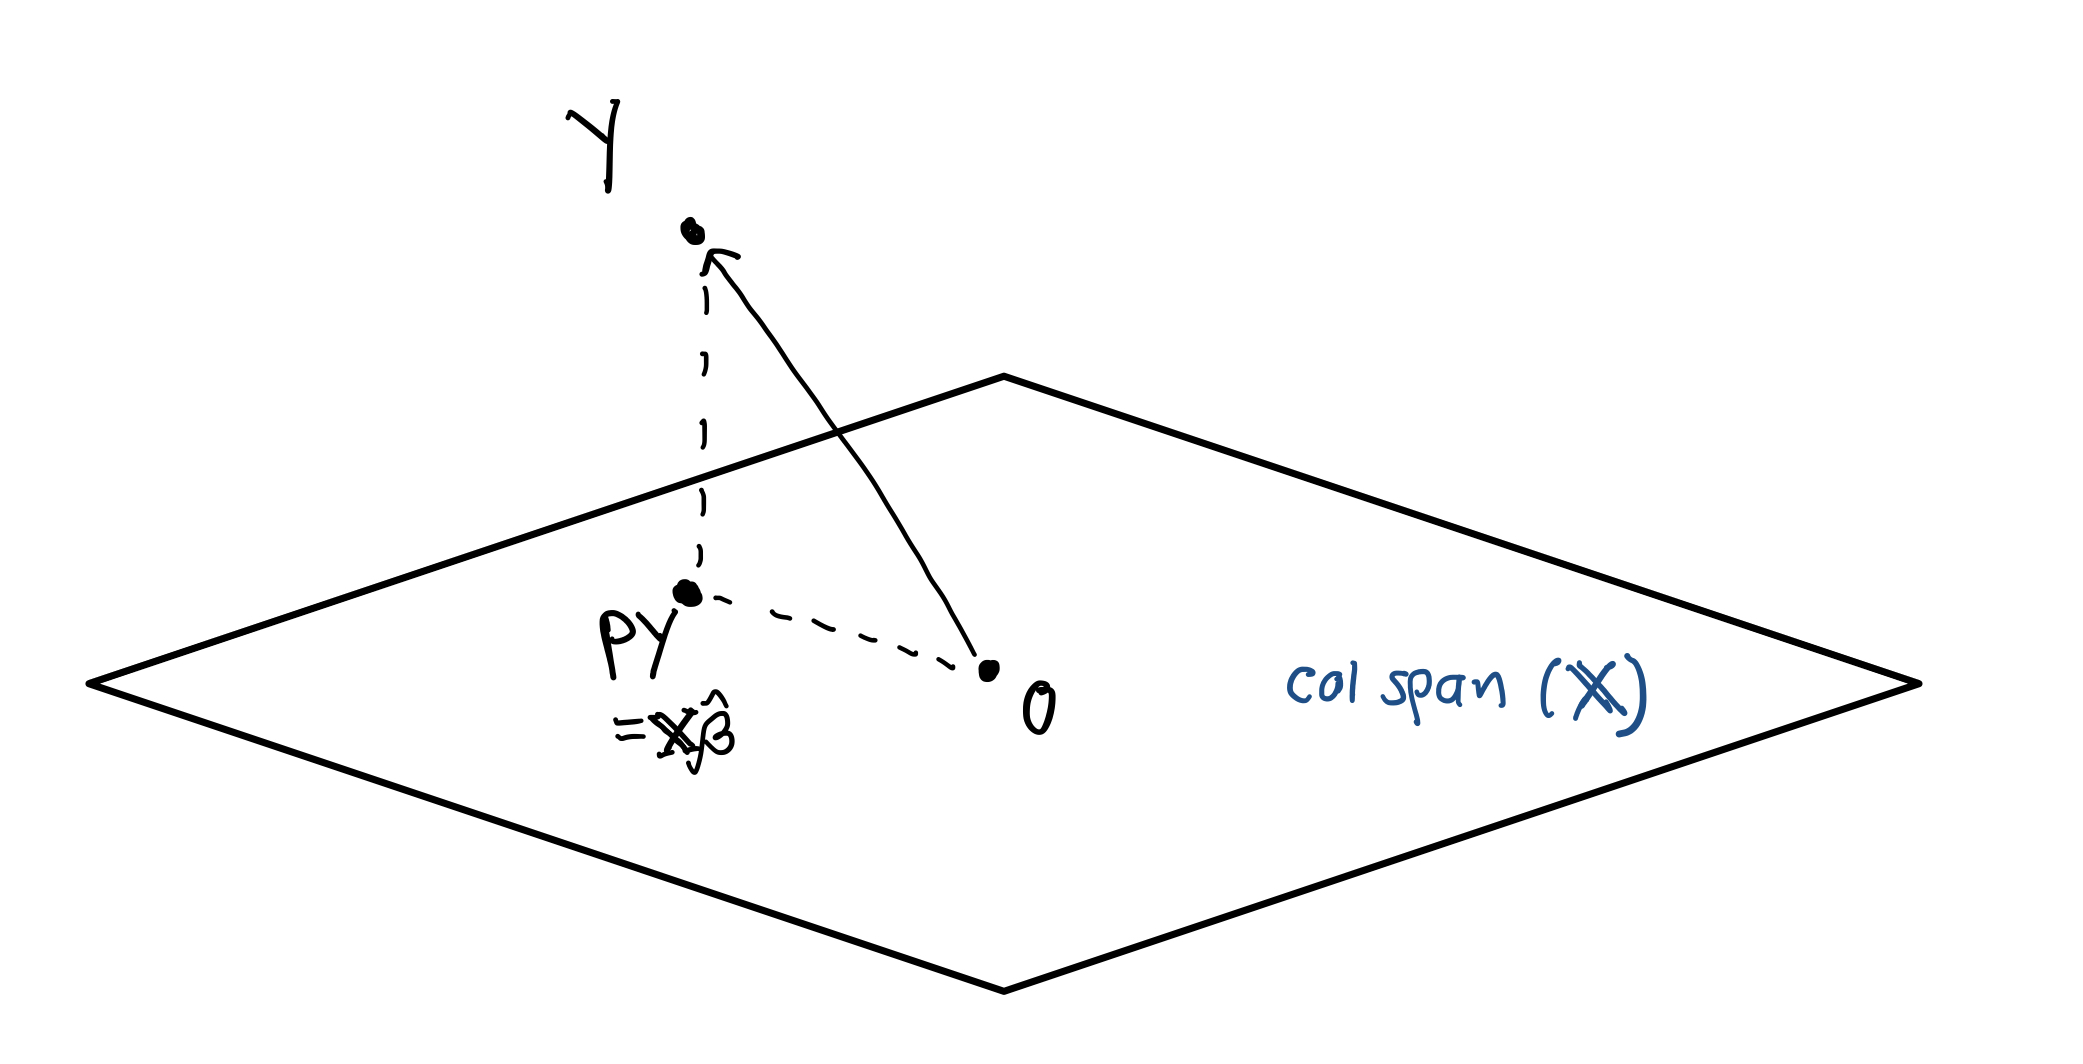
\includegraphics[scale=0.15]{figures/lec3_LSproject.png}
    \caption{Visualization of the least squares solution}
        \label{fig:LS}
\end{figure}



% \section{The Bayes classifier}
% \section{Empirical risk minimization}
% \section{Density-based estimators}
% \section{Regression based classifiers: logistic regression and neural net-
% works}

\end{document}